%!TEX root = 2015-07.tex

\section{Examples}
\subsection{Examples}
\incgraph{../figures/DeepDream/Aurelia-aurita-3/0099.jpg}
\incgraph{../figures/DeepDream/plant/0070.jpg} % TODO
\incgraph{../figures/DeepDream/Sky/0099.jpg}
\incgraph{../figures/Artistic-Style/Aurelia-aurita-3-1-style.jpg}
\incgraph{../figures/Artistic-Style/out-1.jpg}

\begin{frame}{Anwendungen von Machine Learning}
    \begin{itemize}
        \item Spracherkennung: z.B. in Siri (Apple)
        \item Autonome Autos
        \item Einzelhandel: Kundenprofile\footnote{\tiny Kashmir Hill: \enquote{How Target Figured Out A Teen Girl Was Pregnant Before Her Father Did} in Forbes. 16.02.2012.}
        \item Post: Schrifterkennung
        \item Amazon Empfehlungen, Google Suche
        \item Computerspiele: Ego-Shooter, Rennspiele\footnote{\tiny Microsoft Research: \enquote{Playing Machines: Machine Learning Applications in Computer Games}. 05.07.2008 (\href{http://research.microsoft.com/en-us/projects/mlgames2008/}{Link})}
        \item Brettspiele: Backgammon, Go
    \end{itemize}
\end{frame}

\incgraph{../presentation-images/game-ais-xkcd.png}


\section{ML-Basics}
\subsection{ML-Basics}

\begin{frame}{Was ist Machine Learning?}
    \begin{block}{Definition by Tom Mitchell: ML}
        A computer program is said to learn from \textbf{experience} $E$ with
        respect to some class of \textbf{tasks} $T$ and \textbf{performance
        measure} $P$, if its performance at tasks in $T$, as measured by $P$,
        improves with experience $E$.
    \end{block}
\end{frame}

\begin{frame}{MNIST - Ziffern klassifizieren}
    \begin{minipage}[b]{0.45\linewidth}
        \begin{itemize}
            \item Klassen: 0, 1, 2, 3, 4, 5, 6, 7, 8, 9
            \item \num{60000} Trainigsdaten, \num{10000} Testdaten
                  auf \href{http://yann.lecun.com/exdb/mnist/}{yann.lecun.com/exdb/mnist}
            % \item Algorithmen zur Klassifizierung: \textbf{SVMs} (Support Vector Machines),
            %       \textbf{CNNs} (Convolutional Neural Networks),
            %       $k$~Nearest Neighbors (siehe \href{http://martin-thoma.com/k-nearest-neighbor-classification-interactive-example/}{tinyurl.com/knn-interact})
        \end{itemize}
    \end{minipage}
    \hspace{0.5cm}
    \begin{minipage}[b]{0.45\linewidth}
        \begin{figure}
            \centering
            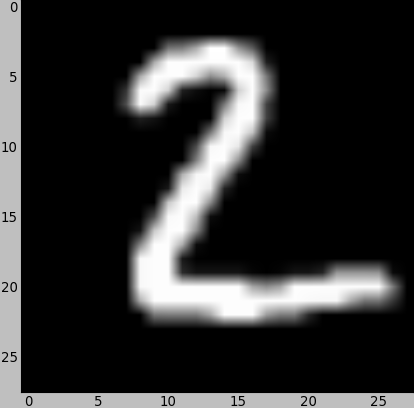
\includegraphics[width=\textwidth]{../presentation-images/mnist-2.png}
            \caption{Datensatz der Klasse \enquote{2}; $\SI{28}{\pixel} \times \SI{28}{\pixel}$}
            \label{fig:spline}
        \end{figure}
    \end{minipage}
\end{frame}

\begin{frame}{Wie löst man das?}
    \begin{itemize}[<+->]
        \item \textbf{Situation}: Daten im $\mathbb{R}^{28 \times 28}$,
              Lösungen in $\Set{0, 1, 2, 3, 4, 5, 6, 7, 8, 9}$
        \item ... oder $[0, 1]^{10}$, wenn wir eine Wahrscheinlichkeitsverteilung wollen
        \item \textbf{Lösung}: Neuronale Netze!
    \end{itemize}
\end{frame}

\section{Neuronale Netze}
\subsection{Neuronale Netze}
\incgraph{../presentation-images/perceptron-unit.pdf}
\incgraph{../presentation-images/feed-forward-perceptron.pdf}

\begin{frame}{}
    \begin{center}
        \Huge Wie finden wir die Gewichte?


        \uncover<2->{Gradientenabstieg (Mehrdimensionale Ableitung)}
    \end{center}
\end{frame}


\begin{frame}{Gradientenabstieg}
    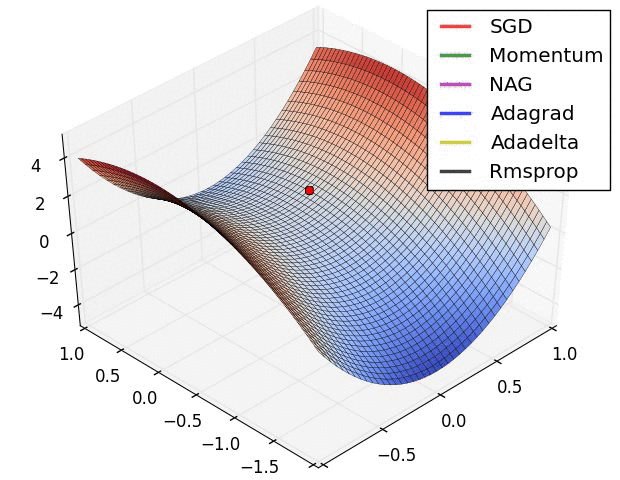
\includegraphics[width=\textwidth, height=0.8\textheight, keepaspectratio]{../presentation-images/visualizing-optimization-algos-0.png}

    Quelle: \href{http://imgur.com/a/Hqolp}{http://imgur.com/a/Hqolp}
\end{frame}


\begin{frame}{}
    \begin{center}
        \Huge Aber wir verlieren die Information, wo etwas ist!

        \uncover<2->{\textbf{Lösung}: Convolutional Neural Networks (CNNs)}
    \end{center}
\end{frame}


\begin{frame}{Image filters}
    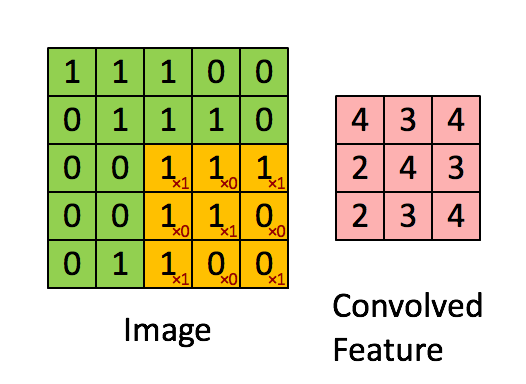
\includegraphics[width=\textwidth, height=0.8\textheight, keepaspectratio]{../presentation-images/image-filter-8.png}

    Quelle: \href{http://ufldl.stanford.edu/wiki/index.php/File:Convolution_schematic.gif}{http://ufldl.stanford.edu/wiki/index.php/File:Convolution\_schematic.gif}
\end{frame}


\begin{frame}{CNNs}
    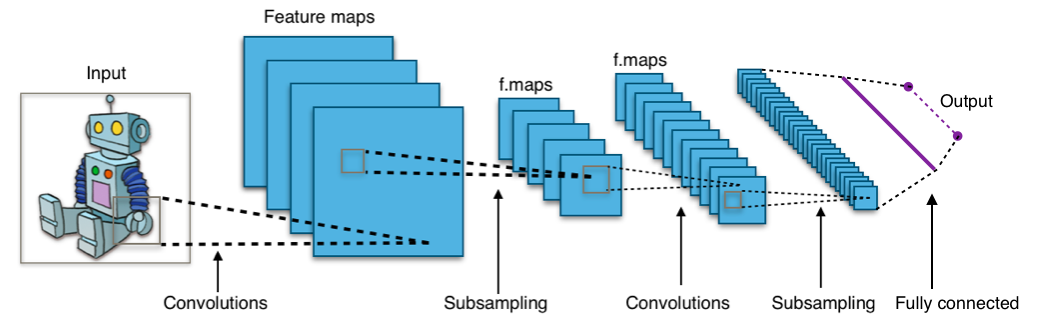
\includegraphics[width=\textwidth, height=0.8\textheight, keepaspectratio]{../presentation-images/Typical-cnn.png}

    Quelle: \href{https://commons.wikimedia.org/wiki/File:Typical_cnn.png}{https://commons.wikimedia.org/wiki/File:Typical\_cnn.png}
\end{frame}

\section{Kreativität}
\subsection{Kreativität}
\begin{frame}{}
    \begin{center}
        \Huge Aber\dots Maschinen sind nicht kreativ!
    \end{center}
\end{frame}
\incgraph{../figures/DeepDream/Aurelia-aurita-3/0099.jpg}
\incgraph{../figures/DeepDream/Aurelia-aurita-3/Aurelia-aurita-3.jpg}
\incgraph{../presentation-images/wired-facebook.png}


\begin{frame}{}
\begin{figure}
\centering
\subfigure[Original Image]{
  \label{fig:scottish-highland-cattle}
  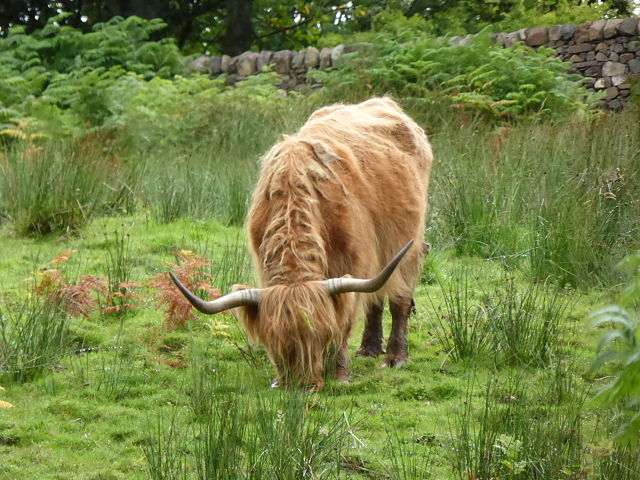
\includegraphics[width=0.45\linewidth, height=0.4\textheight, keepaspectratio]{../figures/Artistic-Style/highland-cattle.jpg}
}%
\subfigure[Style image]{
  \label{fig:starry-night}
  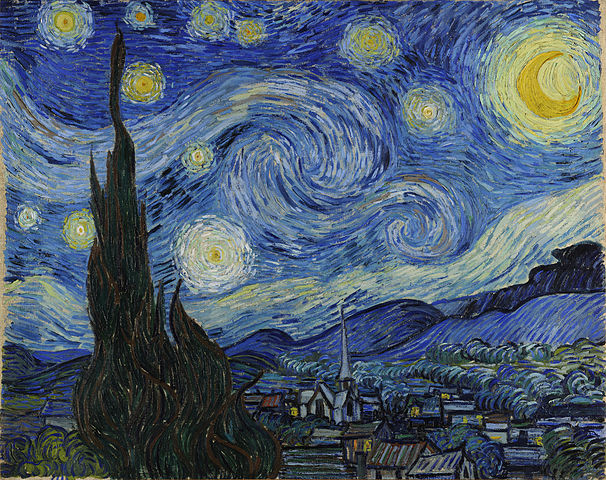
\includegraphics[width=0.45\linewidth, height=0.4\textheight, keepaspectratio]{../figures/Artistic-Style/starry-night.jpg}
}

\subfigure[Result]{
  \label{fig:highland-van-gogh}
  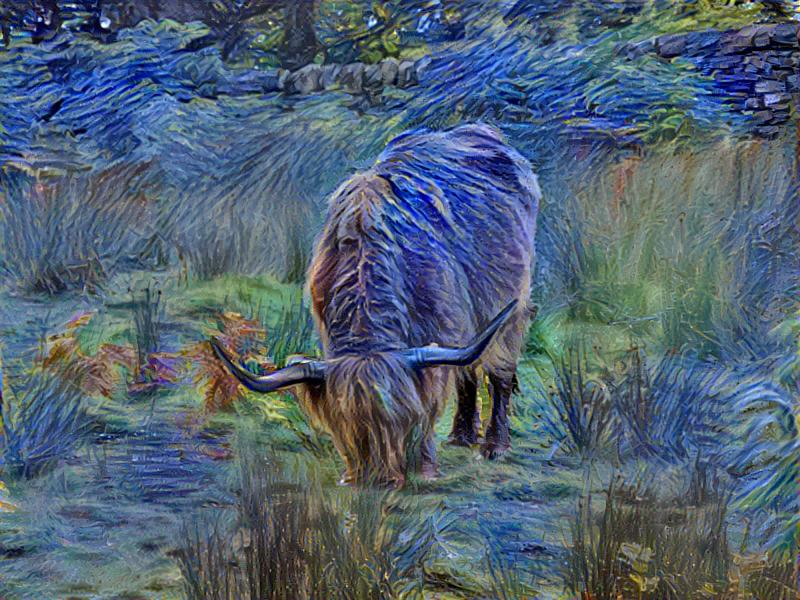
\includegraphics[width=0.93\linewidth, height=0.4\textheight, keepaspectratio]{../figures/Artistic-Style/Scottish-highland-cattle-1-style.jpg}
}
\end{figure}
\end{frame}

\begin{frame}{Neural Style: Schottisches Hochlandrind}
    \begin{center}
        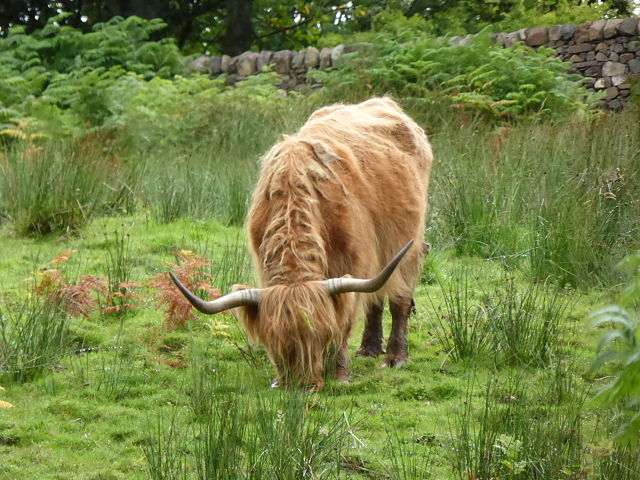
\includegraphics[width=\textwidth, height=0.8\textheight, keepaspectratio]{../figures/Artistic-Style/highland-cattle.jpg}

        Das Original
    \end{center}
\end{frame}

\begin{frame}{Neural Style: Van Goghs \enquote{Starry Night}}
    \begin{center}
        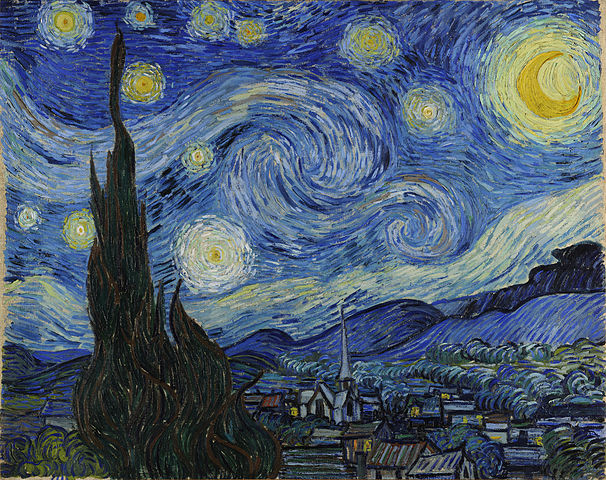
\includegraphics[width=\textwidth, height=0.8\textheight, keepaspectratio]{../figures/Artistic-Style/starry-night.jpg}

    Der Stil des Künstlers
    \end{center}
\end{frame}

\begin{frame}{Das Ergebnis}
    \begin{center}
        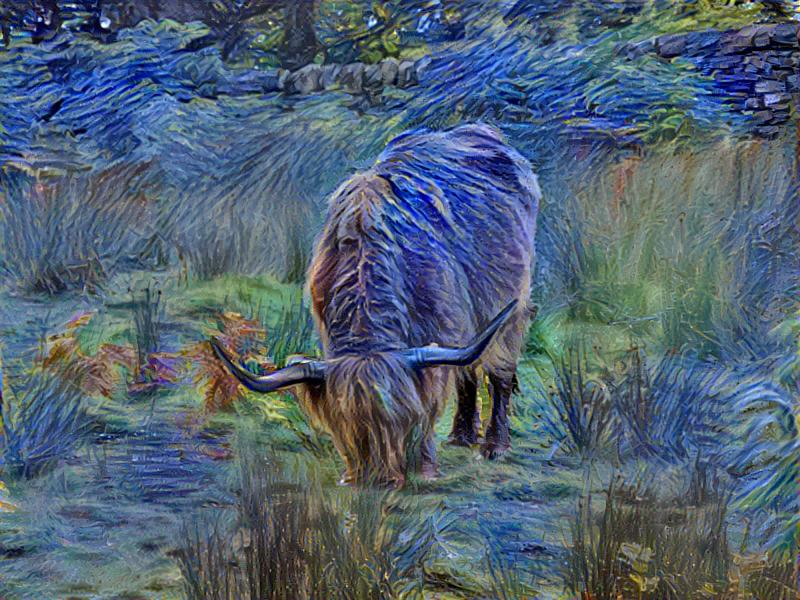
\includegraphics[width=\textwidth, height=0.8\textheight, keepaspectratio]{../figures/Artistic-Style/Scottish-highland-cattle-1-style.jpg}
    \end{center}
\end{frame}


\begin{frame}{}
    \begin{center}
        \Huge Aber\dots Das sind ja nur feste Eingabelängen! Wir Menschen
              können mit Sequenzen umgehen!
    \end{center}
\end{frame}

\begin{frame}{Recurrent Neural Networks (RNNs)}
    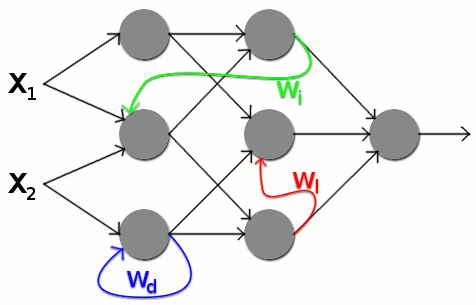
\includegraphics[width=\textwidth, height=0.8\textheight, keepaspectratio]{../presentation-images/recurrrent-neural-networks.png}

    Quelle: \href{https://de.wikipedia.org/wiki/Datei:Neuronal-Networks-Feedback.png}{https://de.wikipedia.org/wiki/Datei:Neuronal-Networks-Feedback.png}
\end{frame}


\begin{frame}{RNN - Shakespeare}
PANDARUS:\\
Alas, I think he shall be come approached and the day
When little srain would be attain'd into being never fed,
And who is but a chain and subjects of his death,
I should not sleep.

Second Senator:\\
They are away this miseries, produced upon my soul,
Breaking and strongly should be buried, when I perish
The earth and thoughts of many states.

DUKE VINCENTIO:\\
Well, your wit is in the care of side and that.

Second Lord:\\
They would be ruled after this chamber, and
my fair nues begun out of the fact, to be conveyed,
Whose noble souls I'll have the heart of the wars.

Clown:\\
Come, sir, I will make did behold your worship.

VIOLA:\\
I'll drink it.
\end{frame}

\begin{frame}{RNN - Wikipedia}
Naturalism and decision for the majority of Arab countries' capitalide was grounded
by the Irish language by [[John Clair]], [[An Imperial Japanese Revolt]], associated
with Guangzham's sovereignty. His generals were the powerful ruler of the Portugal
in the [[Protestant Immineners]], which could be said to be directly in Cantonese
Communication, which followed a ceremony and set inspired prison, training. The
emperor travelled back to [[Antioch, Perth, October 25|21]] to note, the Kingdom
of Costa Rica, unsuccessful fashioned the [[Thrales]], [[Cynth's Dajoard]], known
in western [[Scotland]], near Italy to the conquest of India with the conflict.
Copyright was the succession of independence in the slop of Syrian influence that
was a famous German movement based on a more popular servicious, non-doctrinal
and sexual power post. Many governments recognize the military housing of the
[[Civil Liberalization and Infantry Resolution 265 National Party in Hungary]],
that is sympathetic to be to the [[Punjab Resolution]]
(PJS)[http://www.humah.yahoo.com/guardian.
cfm/7754800786d17551963s89.htm Official economics Adjoint for the Nazism, Montgomery
was swear to advance to the resources for those Socialism's rule,
was starting to signing a major tripad of aid exile.]]
\end{frame}


\section{Fails}
\subsection{Fails}
\begin{frame}{}
    \begin{center}
        \Huge Sind wir (bald) überflüssig?
    \end{center}
\end{frame}

\incgraph{../figures/eth-faces/faces-1.png}
\incgraph{../figures/eth-faces/borat-2-howhot.png}
\incgraph{../figures/eth-faces/borat-3-howhot.png}
\incgraph{../figures/eth-faces/saitama-ok-hot.png}
\incgraph{../figures/eth-faces/thor-godlike-hot.png}
\incgraph{../figures/eth-faces/mr-potato-head-howhot.png}
\incgraph{../figures/eth-faces/how-deep-dream.png}

\begin{frame}{Beispiele}
    Mehr Beispiele gibt es unter

    \begin{itemize}
        \item DeepDream: \href{https://www.reddit.com/r/deepdream/}{reddit.com/r/deepdream}
        \item \#howhot
        \begin{itemize}
            \item \href{https://howhot.io/}{https://howhot.io}
            \item \href{https://www.reddit.com/r/howhot/}{reddit.com/r/howhot}
        \end{itemize}
        \item \href{http://how-old.net/}{how-old.net}
        \item \href{http://write-math.com}{write-math.com}
    \end{itemize}

    \begin{center}
        \Huge Danke für eure Aufmerksamkeit!
    \end{center}
\end{frame}